\section{Desarrollo}

\parencite{molina2013unifying}

\subsection{Descripción del caso práctico}

El estudio presentado propone un controlador difuso unificado para mejorar la gestión de la calidad del ambiente interior (IEQ). Este enfoque busca superar las limitaciones de los sistemas tradicionales de control HVAC, que a menudo son incapaces de manejar de manera eficiente múltiples variables y criterios interrelacionados. 

El caso práctico analizado en la publicación consiste en aplicar el controlador difuso propuesto a una habitación piloto equipada con sensores de temperatura, humedad y calidad del aire. 

\subsection{Diseño del controlador difuso}

La propuesta incluye un controlador basado en lógica difusa, recomendado especialmente en aplicaciones donde el modelo matemático exacto del sistema no es conocido, pero su comportamiento puede ser descrito a partir de la experiencia. Este tipo de controlador mejora la flexibilidad ajustándose a los requisitos de confort y puede manejar situaciones críticas de manera más confiable, gracias a reglas basadas en el conocimiento experto.

\subsubsection{Entradas y salidas}

El sistema utiliza cinco sensores:

\begin{enumerate}
	\item Temperatura interna ($S_{temp_{indoor}}$)
	\item Temperatura externa ($S_{temp_{outdoor}}$)
	\item Humedad relativa ($S_{RH}$)
	\item Concentración de CO2 ($S_{CO_2}$)
	\item Nivel de iluminación ($S_{light}$)
\end{enumerate}

Las salidas son cuatro, que se corresponden a tres actuadores:
\begin{enumerate}
	\item Programa del aire acondicionado ($A_{Air}$): caliente, frío, seco.
	\item Nivel de temperatura ($A_{temp_{level}}$): bajar, mantener, subir.
	\item Nivel de iluminación ($A_{light}$): bajo, medio y alto.
	\item Nivel del humedad ($A_{h_{level}}$): apagado, bajo, estándar, alto, continuo.
\end{enumerate}

Estos actuadores regulan el confort del ambiente interior al influir en el sistema HVAC. Las decisiones sobre estas salidas se toman con base en las lecturas de los cinco sensores y se ajustan dinámicamente según las reglas difusas definidas en el sistema

\subsubsection{Funcionamiento del controlador}

El FLC se basa en un motor de inferencia, que procesa las entradas tras la fuzzificación y genera salidas mediante un proceso de defuzzificación. Esto permite ajustar el sistema para lograr el confort del usuario. REVISAR.

\begin{figure}[H]
	\centering
	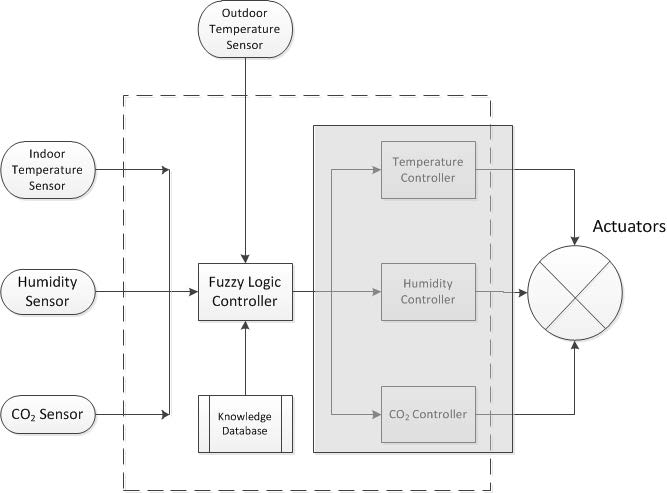
\includegraphics[width=0.85\textwidth]{imgs/arquitectura-FLC.JPG}
	\caption{Arquitectura PID y controlador fuzzy}
	\label{fig:arquitectura-FLC}
\end{figure}

La \autoref{fig:arquitectura-FLC} muestra la arquitectura del FLC, diseñado para regular diferentes variables ambientales mediante un conjunto de sensores y actuadores. Los sensores monitorean parámetros clave, como la temperatura interna y externa, la humedad y la concentración de CO2. Estas lecturas se envían al controlador difuso, que analiza los datos en combinación con una base de conocimiento. Esta base de conocimiento contiene reglas y relaciones definidas por expertos que permiten al sistema tomar decisiones informadas.

El controlador difuso procesa las entradas y determina las acciones necesarias para mantener las condiciones óptimas dentro del entorno. Las decisiones se transmiten a una serie de controladores específicos para cada variable, como el controlador de temperatura, el de humedad y el de CO2. Finalmente, estos controladores ajustan los actuadores correspondientes para implementar las acciones recomendadas. De esta manera, el sistema asegura un ambiente confortable y eficiente, gestionando las interdependencias entre las distintas variables

\vspace{0.4cm}

La \textbf{base de conocimiento} del FLC incluye:
\begin{enumerate}
	\item \textbf{Funciones de membresía}: se utilizan funciones trapezoidales para describir las etiquetas lingüísticas (Bajo, Medio, Alto).
	\begin{figure}[H]
		\centering
		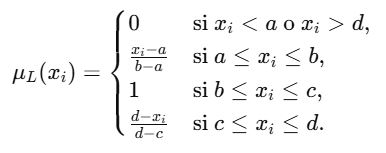
\includegraphics[width=0.55\textwidth]{imgs/function.JPG}
		\caption{Función de membresía}
		\label{fig:function}
	\end{figure}
	
	Se explican algunas variables de la \autoref{fig:function}: $L$ puede tomar el valor de Bajo, Medio y Alto; $a$ y $d$ son los puntos extremos de la función de membresía trapezoidal; $b$ y $c$, los puntos máximos de la función de membresía trapezoidal; y $x_i$ es el $i$-ésimo sensor.
	
	\begin{figure}[H]
		\centering
		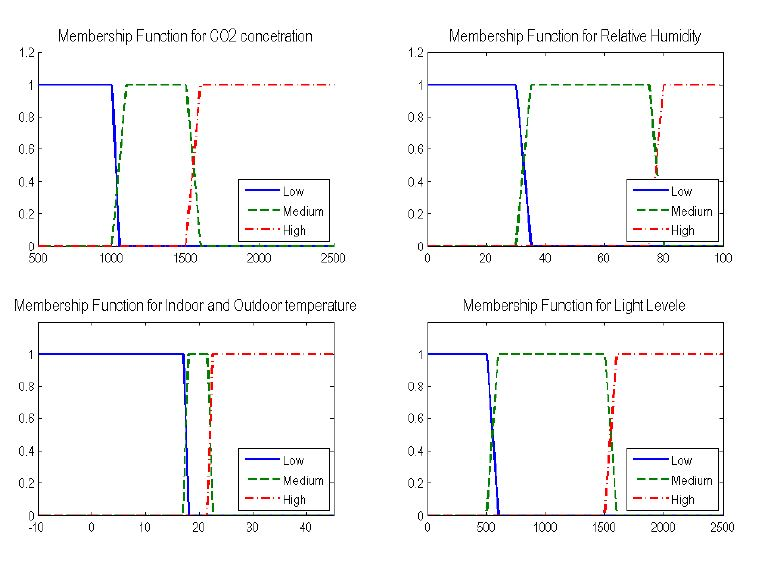
\includegraphics[width=0.8\textwidth]{imgs/membership-functions-input.JPG}
		\caption{Función de membresía de las variables de entrada}
		\label{fig:membership-functions-input}
	\end{figure}
	
	\begin{figure}[H]
		\centering
		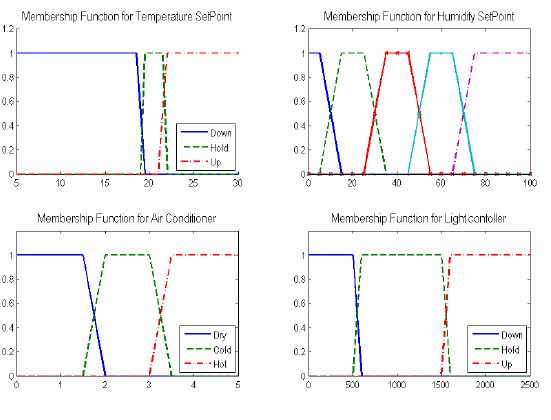
\includegraphics[width=0.8\textwidth]{imgs/membership-functions-output.JPG}
		\caption{Función de membresía de las variables de salida}
		\label{fig:membership-functions-output}
	\end{figure}
	
	\item \textbf{Reglas difusas}: conjunto de reglas IF-THEN derivadas del conocimiento experto. Ejemplos:
	\begin{itemize}
		\item Si la temperatura interna es Media y la externa es Alta, entonces mantener la temperatura y el humidificador en nivel estándar.
		\item Si la humedad es Baja y la temperatura interna es Baja, entonces el aire acondicionado debe estar en caliente, el humidificador en nivel Alto, y subir la temperatura.
	\end{itemize}
	
	Se han utilizado 17 reglas, que dan lugar a diversos escenarios al combinar las posibles entradas del sistema. Se muestra un subconjunto de las reglas en la \autoref{fig:set-of-rules}.
	
	\begin{figure}[H]
		\centering
		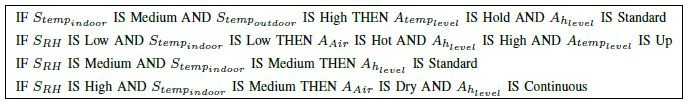
\includegraphics[width=0.9\textwidth]{imgs/set-of-rules.JPG}
		\caption{Conjunto de reglas}
		\label{fig:set-of-rules}
	\end{figure}
	
\end{enumerate}

El motor de inferencia aplica el \textbf{método Mamdani max-min} para combinar reglas y calcular las salidas. Este método evalúa el grado en que cada regla se cumple y combina las salidas difusas.

\begin{figure}[H]
	\centering
	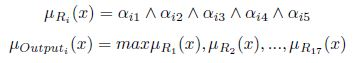
\includegraphics[width=0.50\textwidth]{imgs/mamdani.JPG}
	\caption{Método mamdani max-min}
	\label{fig:mamdani}
\end{figure}

En la \autoref{fig:mamdani}: $x$ son las mediciones de los sensores de entrada, $\alpha_i$ es el grado en que una entrada dada satisface la condición de la $i$-ésima regla ($R_i$), y $\mu_{output_i}$, la agregación de los conjuntos difusos de salida de todas las reglas para $output_i$.

\subsection{Pruebas en simuladores y entornos reales}

\subsubsection{Configuración del simulador}

Se desarrolló un simulador con una interfaz web para probar el controlador difuso que va a gestionar los parámetros de confort ambiental en interiores.

Dicho simulador permite definir rangos de confort, ingresar valores de las condiciones actuales del ambiente (temperatura, iluminación, humedad y concentración de CO2) y obtener las acciones necesarias para mantener dichos parámetros dentro de los rangos deseados.

El simulador contiene tres paneles, asociados a tres elementos distintos:
\begin{enumerate}
	\item \textbf{Los rangos de confort}: este panel permite definir los intervalos de confort que utilizará el controlador para sus reglas difusas. Por ejemplo, se pueden establecer valores específicos para las etiquetas ("baja", "media" y "alta") de humedad o temperatura.
	
	\begin{figure}[H]
		\centering
		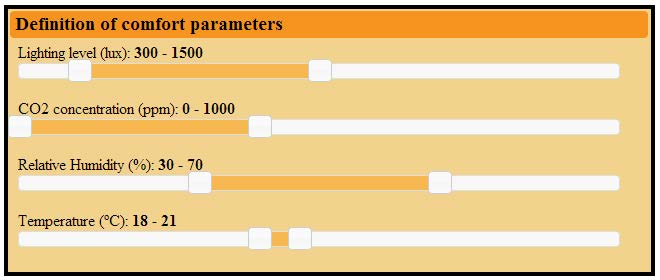
\includegraphics[width=0.6\textwidth]{imgs/simulator-comfort-params.JPG}
		\caption{Panel de definición de intervalos de comfort}
		\label{fig:simulator-comfort-params}
	\end{figure}
	
	\item \textbf{Los valores de entrada}: encargado de registrar los datos de las condiciones de interior actuales, simulando los valores que los sensores reales proporcionarían en un entorno físico real. Estas entradas corresponden a las variables que figuran en los antecedentes de las reglas difusas.
	
	\begin{figure}[H]
		\centering
		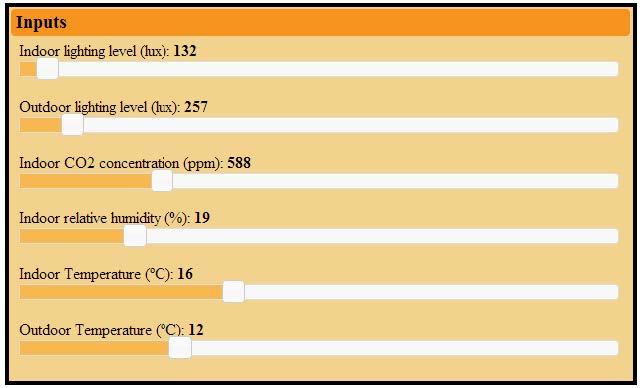
\includegraphics[width=0.6\textwidth]{imgs/simulator-panel-inputs.JPG}
		\caption{Panel de definición de valores de entrada}
		\label{fig:simulator-panel-inputs}
	\end{figure}
	
	\item \textbf{Los valores de salida}: donde se disponen las acciones sugeridas por el controlador para ajustar el ambiente, y así poder reajustar las condiciones actuales dentro de los intervalos de confort definidos en el primer panel.
	
	\begin{figure}[H]
		\centering
		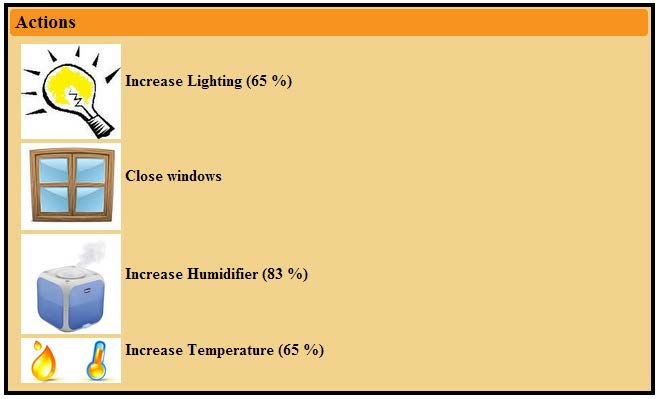
\includegraphics[width=0.6\textwidth]{imgs/simulator-actions-output.JPG}
		\caption{Panel de definición de valores de salida}
		\label{fig:simulator-actions-output}
	\end{figure}
	
	El formato de las salidas son acciones concretas con un grado de aplicación especificado, en el supuesto de que deba aplicarse. A continuación se muestran algunos ejemplos de salidas:
	
	\begin{itemize}
		\item Si la iluminación interior y exterior es baja, se sugiere activar la iluminación artificial.
		\item Si la humedad relativa interior es del 19\%, por debajo del umbral de confort del 30\%, se recomienda activar el humidificador.
		\item Si la temperatura interior es baja y la exterior también, se instruye cerrar las ventanas y aumentar la temperatura usando el sistema HVAC.
	\end{itemize}
	
\end{enumerate}

Los resultados obtenidos concuerdan con las previsiones de los expertos en energía que participaron en el proyecto. Esto demuestra que las reglas implementadas reflejan adecuadamente las estrategias recomendadas para mantener un entorno confortable en interiores. 

Además, el simulador se convirtió en una herramienta útil para la mejora continua, ya que permitió a los expertos realizar ajustes y optimizaciones de manera iterativa. Pues inicialmente, se partió del conjunto de reglas definidas por los expertos, basándose en su conocimiento y experiencia previa; sin embargo, al observar los resultados generados por el simulador en distintos escenarios, pudieron identificar áreas de mejora, logrando así mejorar la precisión del controlador y su capacidad de adaptación a situaciones cambiantes. 

En resumen, el simulador no solo sirvió para validar las reglas iniciales, sino que también actuó como un laboratorio virtual donde los expertos podían experimentar con diferentes configuraciones. Esto permitió un desarrollo progresivo hacia un sistema más robusto, eficiente y alineado con los objetivos de confort y sostenibilidad energética.

\subsubsection{Configuración experimental}

Para complementar las pruebas del simulador previamente mencionado, el controlador difuso fue sometido a una serie de tests en un entorno real, concretamente, en una habitación equipada con varios sensores.

La \textbf{habitación experimental} utilizada, con unas dimensiones de 5.2m x 5.2m x 2.5m, tenía las siguientes características:
\begin{itemize}
	\item Una puerta y una ventana ubicadas en posiciones opuestas.
	\item Un sistema HVAC con calefacción, ventilación y aire acondicionado.
	\item Dos sensores para medir la temperatura y humedad, respectivamente (1).
	\item La ausencia de muebles y ocupantes durante el período de pruebas (2).
\end{itemize}

(1) De esta manera, aunque no pudieron obtenerse resultados en función de todos los parámetros implicados en la IEQ debido a limitaciones técnicas, las dos variables que sí pudieron tomarse en cuenta proporcionaron resultados interesantes.

(2) Para así poder eliminar grandes interferencias externas que pudieran alterar las mediciones; aunque al final la puerta se abrió ocasionalmente, con la entrada breve de algunas personas, lo que terminó generando pequeñas perturbaciones que fueron consideradas en el análisis.

\vspace{0.4cm}

En cuanto a la \textbf{recopilación y almacenamiento de datos}, se tomó el mes de diciembre como período de pruebas, capturando los datos medidos cada 15 minutos. Estas mediciones, que incluían información sobre la temperatura y humedad dentro de la habitación, se exportaron a una base de datos para su posterior análisis y comparación.

\subsection{Resultados del estudio}

Para este subapartado, se han tenido en cuenta los resultados que se obtuvieron en las pruebas experimentales en el período de diciembre de 2012.

Para analizar el rendimiento y utilidad de la propuesta, se realiza una comparación de los resultados obtenidos en la sala piloto cuando se ejecutan dos tipos distintos de controladores: el controlador difuso diseñado y un controlador reactivo más tradicional.

En el caso de la temperatura (\autoref{fig:graph-temperatures-december}), se observa que el controlador difuso, representado en la zona gris del gráfico, logra mantener la temperatura en el rango de confort de manera constante y con mínima variación. Esto significa que el controlador difuso no solo ajusta la temperatura dentro de los límites deseados, sino que también evita grandes fluctuaciones, proporcionando un ambiente estable. En cambio, durante el periodo en blanco, cuando operaba el controlador reactivo, aunque la temperatura también se mantenía en el rango de confort, las oscilaciones eran notoriamente más pronunciadas, lo que implica un ajuste menos preciso y estable.

Para la humedad relativa (\autoref{fig:graph-humidity-december}), aunque la estabilidad es menos clara que en el caso de la temperatura, el controlador difuso también demuestra un mejor rendimiento. En la zona gris, donde el controlador difuso estaba activo, las oscilaciones en la humedad son menores, manteniéndose dentro del rango de confort de forma más controlada. Esto contrasta con el periodo inicial, donde el controlador reactivo produce mayores fluctuaciones, lo que sugiere que el controlador difuso es más efectivo en estabilizar tanto la temperatura como la humedad relativa.

En resumen, estos resultados indican que el controlador difuso no solo es eficaz en mantener las condiciones de confort (temperatura y humedad) dentro de los límites deseados, sino que además logra hacerlo con menos variaciones, creando un ambiente más estable en comparación con el controlador reactivo.

- resumen de resultados

Los resultados obtenidos del estudio indican que el controlador difuso logró mantener las condiciones ambientales dentro de los rangos de confort definidos, con una notable reducción en las fluctuaciones de temperatura y humedad. Durante el período de prueba, el controlador mostró un mejor desempeño que los sistemas reactivos, proporcionando un ambiente más estable y confortable para los ocupantes

- interpretación de los mismos

Estos hallazgos destacan la eficacia del controlador difuso para mejorar la gestión de la calidad ambiental interior. La capacidad del sistema para ajustarse dinámicamente a las condiciones cambiantes del entorno permitió no solo mejorar el confort, sino también optimizar el uso de energía. Esto subraya el potencial de la lógica difusa como una solución integral para sistemas HVAC avanzados en contextos de edificios inteligentes

\begin{figure}[H]
	\centering
	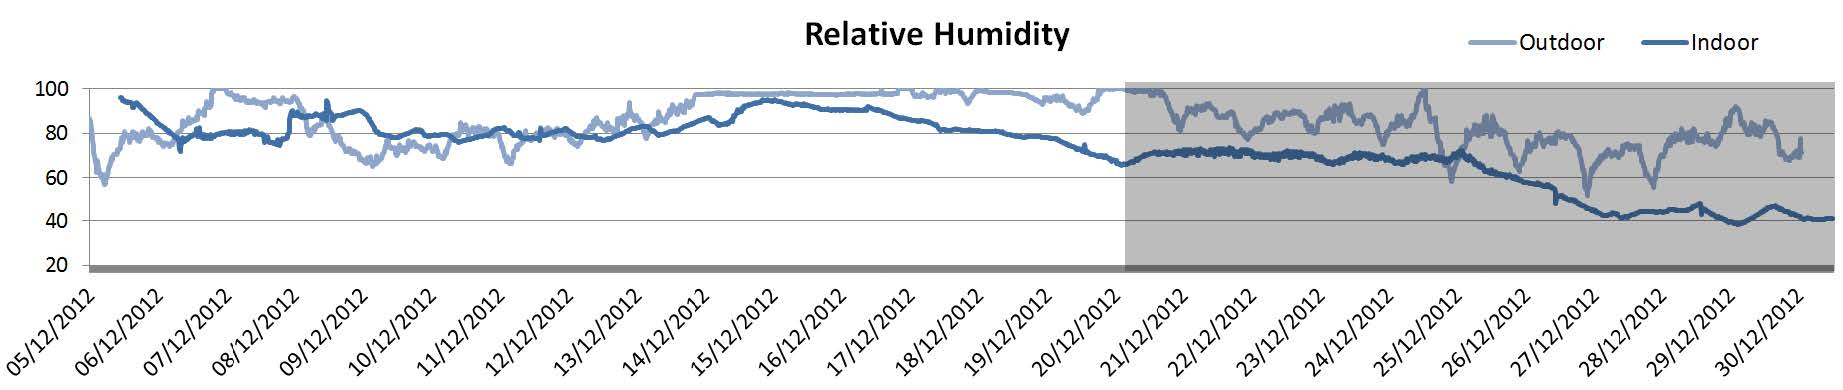
\includegraphics[width=0.95\textwidth]{imgs/graph-humidity-december.JPG}
	\caption{Valores de la humedad recogidos en diciembre de 2012}
	\label{fig:graph-humidity-december}
\end{figure}

\begin{figure}[H]
	\centering
	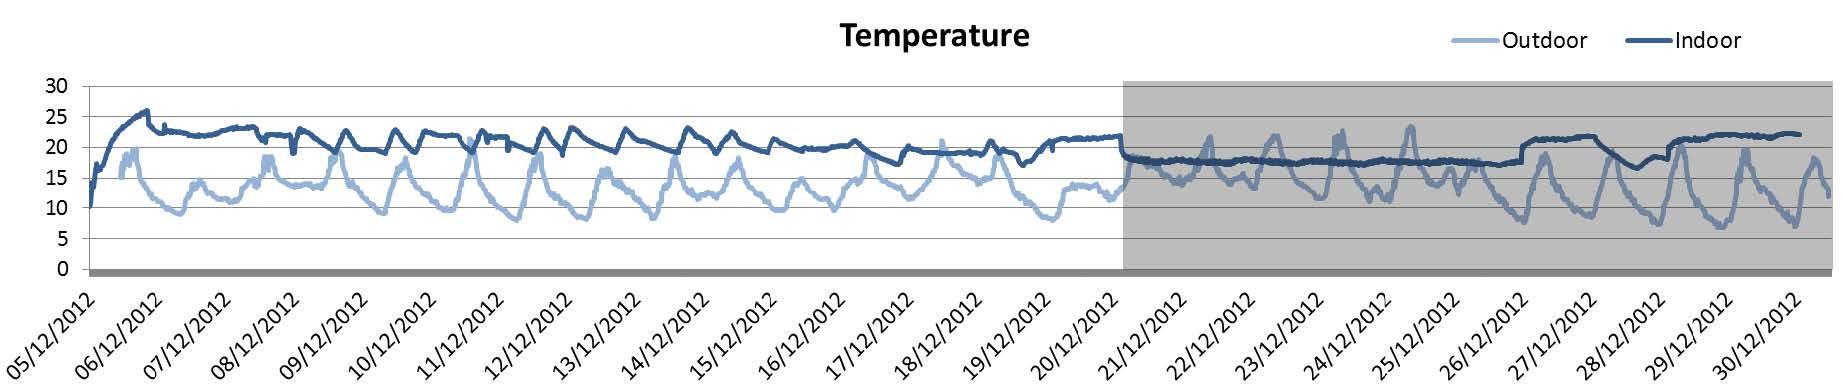
\includegraphics[width=0.95\textwidth]{imgs/graph-temperatures-december.JPG}
	\caption{Valores de la temperatura recogidos en diciembre de 2012}
	\label{fig:graph-temperatures-december}
\end{figure}

